\documentclass[12pt]{article}
\usepackage[utf8]{inputenc}
\usepackage{graphicx}
\graphicspath{{images/}}
\begin{document}
\begin{center}
\huge\underline{SOLUTIONS TO COVID-19 BY}
\huge\underline{BIOMEDICAL ENGINEERS}
\end{center}
\begin{center}
 
\includegraphics[scale=0.7]{nitlogo.png }
\end{center}
\vspace{1cm}
\begin{center}
   \emph{\large By}\\
\Large{ PIYUSH BISEN }\\
\large{Roll No- 21111036}\\
\large{BME 1st Sem}\\
\end{center}
\newpage
\section{Ventilators}
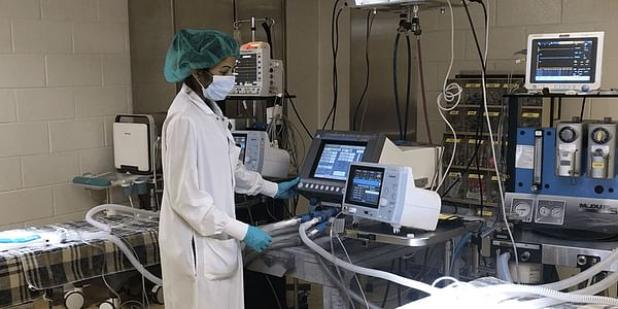
\includegraphics[scale=0.4]{vnt.jpg} 
\\
Patients who cannot breathe spontaneously need to be put on a ventilator.
Ventilators are capable of replacing the breath function and patients in an
advanced state of respiratory distress are usually intubated and sedated at
the beginning of the treatment.
Ventilators are capable of replacing the breath function and patients in
an advanced state of respiratory distress are usually intubated and sedated
at the beginning of the treatment. They are complex systems providing
the healthcare professionals with a lot of flexibility to adapt the assisted
breathing settings and to be able to wean recovering patients off the ventilator
gradually.
Modern ventilators are typically closed loop pressure controlled and capable of detecting spontaneous breathing to synchronise assistance for recovering patients. They also enable the control of the composition of the gas
the patient breathes from normal air to 100 percent oxygen, usually taking
their supply from the hospital’s gas supply network but can also be coupled
to oxygen tanks or oxygen concentrators if used in a setting where there is
no gas network.
\section{Biomedical Engineers’ rapid response to PPE needs}
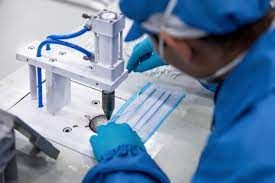
\includegraphics[scale=0.65]{ppe.jpeg} 
\\
According to infectious disease experts, face shields protect the face from
fluids, spray, and droplets, while extending the life of N95 face masks.
The COVID-19 pandemic has depleted supplies of personal protective equipment (PPE) for healthcare professionals nationwide. Dr. Karilyn Larkin is a
hematologist at The Ohio State University Comprehensive Cancer Center –
Arthur G. James Cancer Hospital and Richard J. Solove Research Institute.
When she and her colleagues experienced shortages of face shields, she turned
to Ohio State engineers—specifically Mechanical and Aerospace Engineering
Professor Carlos Castro—for help 3D printing face shields.
\section{Mental Health}

\includegraphics[scale=0.65]{mh.jpeg}
\\
People are expected to quarantine and self-isolate, closing themselves off
socially, as the number of mental health concerns rises amid the Covid-19
health crisis.
For overcoming this many apps were developed like covid coach .
Even many people were using AR and VR for their entertainment
purpose. Doing exercise and yoga to keep themselves fit and while doing
this the smart watch records all their biological activities for tracking
their health
\section{Testing and Tracking}
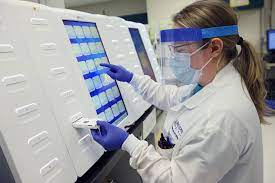
\includegraphics[scale=0.65]{tt.jpeg} 
\\
When covid-19 pandemic ocured we needed as many testing kits as
possible to tackle the virus.It includes rapid tests which took short time
to declare the results as compared to pcr tests.
Because of the risk of infection and quick transmission, the development
of software and technical applications, such as telemedicine to watch the
virus’s evolution in the population, has gotten a lot of interest.
Many testing kits were developed by the engineers.
Like :
\\
\\
Smart iot covid-19 automator test booth hello for paperless and registration and online sample linking.
\section{Vaccines}
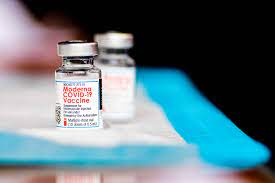
\includegraphics[scale=0.65]{vcn.jpeg}
\\
The labs of Biomedical Engineering Professors Daniel Gallego-Perez and Natalia Higuita-Castro are developing novel, highly benign and targeted meth4
ods for the delivery of mRNA vaccines. While the researchers normally focus
on cancer and regenerative medicine, their methods may be applicable to
vaccine development and deployment.

\end{document}